\documentclass[10pt, a4paper]{article}

% ── Packages ──────────────────────────────────────────────────────────
\usepackage[margin=1.3cm]{geometry}
\usepackage{amsmath, amssymb}
\usepackage{graphicx}
\usepackage{booktabs}
\usepackage{multirow}
\usepackage{caption}
\usepackage{subcaption}
\usepackage[hidelinks]{hyperref}
\usepackage{enumitem}
\usepackage{float}
\usepackage{tikz}
\usetikzlibrary{positioning, arrows.meta, fit, calc, shapes.geometric}
\usepackage{xcolor}
\usepackage[numbers]{natbib}
\usepackage{setspace}
\onehalfspacing

% ── Macros ────────────────────────────────────────────────────────────
\newcommand{\cindex}{C\text{-index}}

\definecolor{staticblue}{HTML}{5C6BC0}
\definecolor{tsgreen}{HTML}{26A69A}
\definecolor{textorange}{HTML}{FF7043}
\definecolor{fusionred}{HTML}{EF5350}
\definecolor{highlight}{RGB}{248, 231, 230}

\title{\textbf{Multi-Modal Deep Learning for ICU Time-to-Discharge Prediction:\\A Landmark Dynamic Survival Analysis Approach}}
\author{SPH6004 Group Assignment}
\date{April 2026}

\begin{document}
\maketitle


% ══════════════════════════════════════════════════════════════════════
\section{Problem Statement}
\label{sec:problem}
% ══════════════════════════════════════════════════════════════════════

Predicting the continuous time-to-discharge for patients in the Intensive Care Unit (ICU) is a critical survival analysis task that supports bed management and proactive care planning. Early approaches to ICU time-to-discharge prediction primarily utilised single-modality clinical data---such as tabular admission demographics or basic physiological time-series. However, these methods suffer from two major limitations: they fail to extract the nuanced prognostic reasoning embedded within unstructured clinical texts, and they typically generate only a single forecast upon admission, which quickly becomes obsolete as a patient's condition evolves. To overcome these critical flaws, this paper proposes a \textbf{multi-modal deep survival model} integrated within a \textit{landmark dynamic prediction framework}. Implemented via dynamic sample generation, the dataset is dynamically cohorted at three specific prediction time points ($t \in \{24, 48, 72\}$ hours). At each landmark, only patients whose observed length of stay exceeds the landmark hour are evaluated. This allows the model to explicitly condition its discrete-time survival predictions on the unfolding clinical trajectory up to that exact hour.


% ══════════════════════════════════════════════════════════════════════
\section{Data Description}
\label{sec:data}
% ══════════════════════════════════════════════════════════════════════

This study utilizes the MIMIC-IV (v3.1) database to predict the continuous time-to-discharge for ICU survivors. To address the complexities of clinical outcomes, we employ a competing-risk survival analysis framework. Within this framework, a living ICU discharge is defined as the primary event of interest ($\delta = 1$), while in-hospital or intra-ICU mortality is treated as a right-censored observation ($\delta = 0$). This design ensures the model prioritizes the recovery trajectory of survivors while accounting for death as a terminal event that prevents discharge.

To capture the evolving clinical states of critically ill patients, we adopt a dynamic landmarking paradigm ($t_{\text{obs}} \in \{24, 48, 72\}$ hours), integrating multi-modal evidence available up to each specific landmark:

\begin{itemize}
    \item \textbf{Static Context:} Time-invariant demographics and admission-time features (107 features after preprocessing).
    \item \textbf{Physiological Dynamics:} Longitudinal time-series measurements reflecting acute physiological responses (22 per-hour channels).
    \item \textbf{Clinical Narratives:} Unstructured radiology and nursing notes containing nuanced prognostic reasoning.
\end{itemize}

The selection of $t_{obs} \in \{24, 48, 72\}$ hours as our primary landmark points is informed by both methodological standards and clinical practice. According to the landmarking framework established by van Houwelingen \cite{vanhouwelingen2007dynamic}, these time points are strategically chosen to capture meaningful shifts in the hazard rate as new clinical information accrues. In the ICU context, the 24 to 72-hour window represents a critical "stabilization window" where initial acute interventions are completed and treatment responses become observable. By generating predictions at these specific intervals, we align our model with standard clinical review cycles—where physicians typically reassess discharge readiness—while ensuring a sufficient accumulation of longitudinal data to provide high-confidence prognostic updates.


The cohort was refined by removing 10 leakage/identifier columns and 34 features with high missingness ($>60\%$). The final study cohort comprises 76,943 ICU stays from 53,569 unique subjects. The dataset exhibits an alive discharge rate of 92.7\%, with the remaining 7.3\% representing ICU mortality (censoring). The framework ultimately processes over 3.6 million rows of time-series data to generate updated survival probabilities reflecting the most recent clinical status.


\begin{table}[h]
\centering
\caption{Dataset overview after cohort construction.}
\label{tab:data_overview}
\begin{tabular}{llr}
\toprule
\textbf{Property} & \textbf{Detail} & \textbf{Value} \\
\midrule
ICU stays & Total cohort & 76{,}943 \\
Unique subjects & & 53{,}569 \\
Alive discharge rate & & 92.7\% \\
ICU death (censoring) rate & & 7.3\% \\
\midrule
\multirow{3}{*}{Eligible stays by landmark} & $t = 24$ h & 60{,}687 \\
& $t = 48$ h & 36{,}911 \\
& $t = 72$ h & 24{,}413 \\
\midrule
Static features (after preprocessing) & Numeric + OHE & 107 \\
Time-series features & Per-hour channels & 22 \\
Time-series total rows & & 3{,}658{,}637 \\
\bottomrule
\end{tabular}
\end{table}


% ══════════════════════════════════════════════════════════════════════
\section{Methodology}
\label{sec:methods}
% ══════════════════════════════════════════════════════════════════════

\subsection{Problem Formulation: Landmark Dynamic Survival Analysis}
\label{subsec:landmark_dynamic}

Let $T_{total}$ represent the continuous overall length of stay for an ICU patient and $t_{obs} \in \{24, 48, 72\}$ denote the predefined observation landmark times. We filter the cohort such that only patients who survive and remain in the ICU beyond $t_{obs}$ (i.e., $T_{total} > t_{obs}$) are included in the prediction task. 

The predictive target is the residual length of stay, defined as:
\begin{equation}
    T_{res} = T_{total} - t_{obs}
\end{equation}

Let $C$ denote the censoring time. The observed time $Y$ and the event indicator $\delta$ are defined as:
\begin{equation}
    Y = \min(T_{res}, C)
\end{equation}
\begin{equation}
    \delta = I(T_{res} \le C)
\end{equation}
where $\delta = 1$ indicates a living ICU discharge (the event of interest) and $\delta = 0$ indicates right-censoring due to in-hospital or intra-ICU mortality.

At each landmark $t_{obs}$, our multi-modal neural network framework utilizes the heterogeneous clinical data collected up to $t_{obs}$, denoted as $\mathbf{X}(t_{obs})$, to estimate the conditional survival function. The continuous survival function is defined as the probability that the residual length of stay $T_{res}$ exceeds a given time $t$:
\begin{equation}
    S(t \mid \mathbf{X}(t_{obs})) = P(T_{res} > t \mid \mathbf{X}(t_{obs}), T_{total} > t_{obs})
\end{equation}

To adapt this to our discrete-time neural network architecture (e.g., DeepHit), the continuous time horizon is partitioned into $K$ discrete intervals. The model is trained to output a Probability Mass Function (PMF), where $p_k(\mathbf{X}(t_{obs})) = P(T_{res} \in \text{bin}_k \mid \mathbf{X}(t_{obs}))$ represents the probability of the event (living discharge) occurring specifically within the $k$-th interval. Consequently, the discrete survival function $S(t_k)$ evaluated at the upper bound of interval $k$ is computationally derived by accumulating the event probabilities:
\begin{equation}
    S(t_k \mid \mathbf{X}(t_{obs})) = 1 - \sum_{j=1}^{k} p_j(\mathbf{X}(t_{obs}))
\end{equation}

\subsection{Data Preprocessing}
\subsubsection{Splitting, Sample Weighting, and Static Processing}
To ensure patient-level isolation, we applied a 5-fold Stratified Group K-Fold split based on \texttt{subject\_id}. Furthermore, because the dynamic landmarking approach inherently generates multiple samples (e.g., at 24h, 48h, and 72h) for patients with longer ICU stays, we applied an inverse frequency sample weighting strategy ($w = 1.0 / N_{\text{samples per subject}}$). This explicitly down-weights patients with extended stays, preventing them from disproportionately dominating the model training. 

From 142 raw static features, leakage-prone and high-missingness columns were removed. Gender was binarized, race collapsed into 5 groups, and other categorical variables one-hot encoded (\texttt{handle\_unknown='ignore'}). Missing values were imputed via a distance-weighted K-nearest-neighbour imputer ($k = 10$). Finally, features were standardized using \texttt{StandardScaler} fitted exclusively on training data, yielding 107-dimensional static feature vectors.

\subsubsection{Time-Series Processing}
Excluding two channels with 100\% missingness (\texttt{spo2}, \texttt{inr}), 22 essential features (e.g., vitals, labs, SOFA scores) were retained. Measurements were filtered to the $(-1, 72)$ hour interval relative to admission. We computed binary observation masks for each feature. Per-fold Z-score normalization ($\epsilon = 10^{-8}$) was applied using training statistics, filling unobserved values with zero. The final input is a $(72, 44)$-dimensional tensor (22 value channels concatenated with 22 masks).

The explicit concatenation of observation masks is a critical design choice. Because missing values are zero-imputed post-normalization, the mask allows the model to distinguish between a true unobserved value and an actual clinical measurement that equals the population mean (which normalizes to zero). Furthermore, clinical missingness is highly informative—the frequency of ordered tests inherently encodes the clinician's suspicion and the patient's acuity. This masking strategy aligns with established methodologies for modeling highly sparse multivariate clinical time-series, which has been shown to significantly enhance predictive performance \cite{lipton2016directly, che2018recurrent}.

\subsubsection{Text Processing and Target Discretization}
Radiology reports were de-identified with \texttt{[DEID]} tokens, keeping only notes where $t < t_{obs}$. High-value sections (CONCLUSION, etc.) were prioritized. Text was truncated via head-tail windowing: 192 head/64 tail words for summaries; 96 head/160 tail for non-summary text. Tokenization utilized ClinicalBERT (max length 256) to extract semantic embeddings. Finally, $T_{res}$ was discretized into $K$ bins using training-derived quantile boundaries to ensure balanced event distributions.


\subsection{Model Architecture}
\label{sec:architecture}

The proposed multi-modal architecture consists of three modality-specific encoders, a pairwise cross-attention fusion mechanism, a fusion MLP, and a discrete survival prediction head. Figure~\ref{fig:architecture} provides an overview of the full pipeline.

\begin{figure}[htbp]
\centering
% 使用 resizebox 使其自动适配单栏或双栏页宽，防止溢出边缘
\resizebox{\linewidth}{!}{%
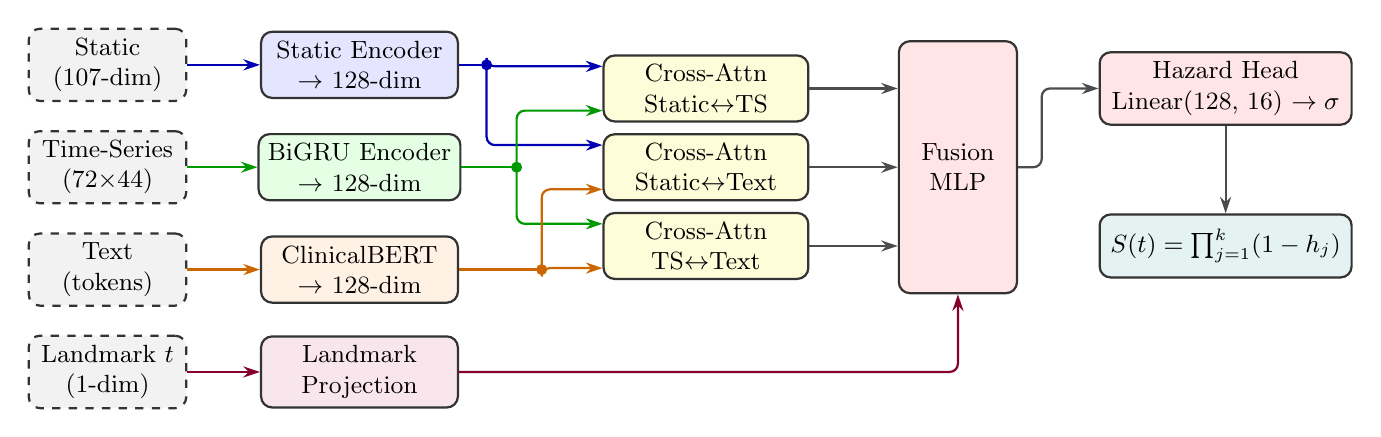
\begin{tikzpicture}[
    % 现代扁平化方块样式
    block/.style={rectangle, draw=black!80, thick, rounded corners=4pt, minimum height=0.8cm, align=center, font=\small},
    data/.style={block, fill=gray!10, dashed, minimum width=2.0cm},
    encoder/.style={block, minimum width=2.5cm},
    attn/.style={block, fill=yellow!15, minimum width=2.6cm},
    % Fusion MLP 设为长条形，完美覆盖并收集所有注意力特征
    fusion/.style={block, fill=red!10, minimum height=3.2cm, minimum width=1.5cm},
    % 标准连线与箭头样式
    arr/.style={-{Stealth[length=6pt, width=4pt]}, thick, color=black!70, rounded corners=3pt},
]

% ==================== 1. 定义专属模态颜色 ====================
% 使用不同颜色渲染排线，彻底解决线条交叉时的视觉混淆
\colorlet{sColor}{blue!70!black}
\colorlet{tColor}{green!60!black}
\colorlet{xColor}{orange!80!black}
\colorlet{lColor}{purple!70!black}

\tikzset{
    s_arr/.style={-{Stealth[length=6pt, width=4pt]}, thick, color=sColor, rounded corners=3pt},
    t_arr/.style={-{Stealth[length=6pt, width=4pt]}, thick, color=tColor, rounded corners=3pt},
    x_arr/.style={-{Stealth[length=6pt, width=4pt]}, thick, color=xColor, rounded corners=3pt},
    l_arr/.style={-{Stealth[length=6pt, width=4pt]}, thick, color=lColor, rounded corners=3pt},
}

% ==================== 2. 定义严格对齐的 Y 轴网格 ====================
\def\yS{0}
\def\yT{-1.3}
\def\yX{-2.6}
\def\yL{-3.9}

% 错位插入的 Attention 层高度

\def\yCAone{-0.30}
\def\yCAtwo{-1.30}
\def\yCAthree{-2.30}

% ==================== 3. 数据输入层 (X = 0) ====================
\node[data] (static_in) at (0, \yS) {Static\\(107-dim)};
\node[data] (ts_in)     at (0, \yT) {Time-Series\\(72$\times$44)};
\node[data] (text_in)   at (0, \yX) {Text\\(tokens)};
\node[data] (lm_in)     at (0, \yL) {Landmark $t$\\(1-dim)};

% ==================== 4. 特征编码层 (X = 3.2) ====================
\node[encoder, fill=blue!10]   (enc_s) at (3.2, \yS) {Static Encoder\\$\to$ 128-dim};
\node[encoder, fill=green!10]  (enc_t) at (3.2, \yT) {BiGRU Encoder\\$\to$ 128-dim};
\node[encoder, fill=orange!10] (enc_x) at (3.2, \yX) {ClinicalBERT\\$\to$ 128-dim};
\node[encoder, fill=purple!10] (enc_l) at (3.2, \yL) {Landmark\\Projection};

\draw[s_arr] (static_in) -- (enc_s);
\draw[t_arr] (ts_in)     -- (enc_t);
\draw[x_arr] (text_in)   -- (enc_x);
\draw[l_arr] (lm_in)     -- (enc_l);

% ==================== 5. 交叉注意力层 (X = 7.6) ====================
\node[attn] (ca1) at (7.6, \yCAone)   {Cross-Attn\\Static$\leftrightarrow$TS};
\node[attn] (ca2) at (7.6, \yCAtwo)   {Cross-Attn\\Static$\leftrightarrow$Text};
\node[attn] (ca3) at (7.6, \yCAthree) {Cross-Attn\\TS$\leftrightarrow$Text};

% ==================== 6. 彩色数据流总线 (Buses) ====================
% 设立三个不同深度的中转 X 坐标，形成电路板级别的极客排线槽
\path (enc_s.east) -- ++(0.35,0) coordinate (s_bus);
\path (enc_t.east) -- ++(0.70,0) coordinate (t_bus);
\path (enc_x.east) -- ++(1.05,0) coordinate (x_bus);

\draw[thick, color=sColor] (enc_s.east) -- (s_bus);
\draw[thick, color=tColor] (enc_t.east) -- (t_bus);
\draw[thick, color=xColor] (enc_x.east) -- (x_bus);

% 添加实心交汇点，使分流逻辑更加清晰
\fill[sColor] (s_bus) circle (2pt);
\fill[tColor] (t_bus) circle (2pt);
\fill[xColor] (x_bus) circle (2pt);

% Static 蓝色特征流 (分别接入 ca1 和 ca2 上端)
\draw[s_arr] (s_bus) |- ([yshift=8pt]ca1.west);
\draw[s_arr] (s_bus) |- ([yshift=8pt]ca2.west);

% Time-Series 绿色特征流 (分别接入 ca1 下端 和 ca3 上端)
\draw[t_arr] (t_bus) |- ([yshift=-8pt]ca1.west);
\draw[t_arr] (t_bus) |- ([yshift=8pt]ca3.west);

% Text 橙色特征流 (分别接入 ca2 下端 和 ca3 下端)
\draw[x_arr] (x_bus) |- ([yshift=-8pt]ca2.west);
\draw[x_arr] (x_bus) |- ([yshift=-8pt]ca3.west);

% ==================== 7. 特征融合层 (X = 10.8) ====================
\node[fusion] (fuse) at (10.8, \yCAtwo) {Fusion\\MLP};

% 统一汇总：使用标准灰色线将 Attention 汇入 Fusion
\draw[arr] (ca1.east) -- (ca1.east -| fuse.west);
\draw[arr] (ca2.east) -- (fuse.west);
\draw[arr] (ca3.east) -- (ca3.east -| fuse.west);

% Landmark 紫色特征由底部绕行，完美无障碍托底直角汇入 Fusion 底部
\draw[l_arr] (enc_l.east) -| (fuse.south);

% ==================== 8. 预测头与损失层 (X = 14.2) ====================
% 将最后两个组件上下折叠排布，大幅节约宽度空间
\node[block, fill=red!10, minimum width=3.2cm]  (head) at (14.2, \yCAone)   {Hazard Head\\Linear(128, 16) $\to \sigma$};
\node[block, fill=teal!10, minimum width=3.2cm] (surv) at (14.2, \yCAthree) {$S(t) = \prod_{j=1}^{k}(1-h_j)$};

% 直角排线连接输出
\draw[arr] (fuse.east) -- ++(0.3,0) |- (head.west);
\draw[arr] (head.south) -- (surv.north);

\end{tikzpicture}%
}
\caption{Architecture of the multi-modal discrete-time survival model. Three modality-specific encoders produce 128-dimensional representations, fused via pairwise cross-attention and an MLP to predict per-bin hazard probabilities.}
\label{fig:architecture}
\end{figure}

\subsubsection{Landmark Time Integration}
As detailed in Section~\ref{subsec:landmark_dynamic}, we conduct dynamic length-of-stay prediction at three pre-defined landmark times: 24, 48, and 72 hours after ICU admission. To enable the model to adapt its prediction strategy to different stages of a patient’s ICU stay, we explicitly incorporate the landmark time as a learnable feature in the multi-modal fusion pipeline.Specifically, the normalized landmark time is projected into the shared latent space and concatenated with the modality-specific representations and pairwise cross-attention features before fusion. This design ensures the model maintains temporal awareness, accounting for time-varying patterns in patient acuity, data availability, and remaining stay dynamics across different landmark points. By conditioning predictions on the elapsed time since admission, the model aligns with real-world clinical decision-making workflows, where updated forecasts are generated at regular intervals throughout a patient’s ICU stay.

The proposed multi-modal architecture consists of three modality-specific encoders, a pairwise cross-attention fusion mechanism, a fusion MLP, and a discrete survival prediction head. Figure~\ref{fig:architecture} provides an overview of the full pipeline.


\subsubsection{Static Encoder}

The static encoder is a two-layer feed-forward network: $\text{Linear}(107, 256) \to \text{LayerNorm} \to \text{ReLU} \to \text{Dropout}(0.3) \to \text{Linear}(256, 128) \to \text{ReLU}$. This network maps the 107-dimensional preprocessed static feature vector to a 128-dimensional dense embedding, capturing non-linear relationships between baseline admission characteristics.

\subsubsection{Time-Series Encoder (Bidirectional GRU)}

Hourly time-series data is encoded using a 2-layer bidirectional GRU with hidden dimension 128 per direction. The input to the GRU concatenates 22 feature values with their 22 binary observation masks, resulting in a 44-dimensional input at each timestep. This mask concatenation is a deliberate design choice: it enables the GRU to distinguish between a measured zero value and an unobserved/missing measurement, which is critical given the high sparsity of ICU time-series data. Variable-length sequences are handled via PyTorch's \texttt{pack\_padded\_sequence} utility, with zero-filled outputs for samples with no valid time-series observations before the landmark. The encoder produces two outputs:
\begin{itemize}[nosep]
    \item A \textit{sequence output} projected to 128 dimensions via $\text{Linear}(256, 128)$(used for cross-attention),
    \item A \textit{summary vector} from the summary vector from the concatenated final forward and backward hidden states, projected to 128 dimensions via $\text{Linear}(256, 128)$.
\end{itemize}

\subsubsection{Text Encoder (ClinicalBERT)}

We employ ClinicalBERT \citep{alsentzer2019clinicalbert}, a BERT model pre-trained on clinical notes from the MIMIC-III database, for radiology report encoding. All BERT parameters are \textbf{frozen} during training to prevent overfitting, given the limited temporally-safe text supervision signal (only $\sim$23{,}000 temporally-safe training samples per fold out of $\sim$122{,}000 dynamic samples). A learnable projection layer ($\text{Linear}(768, 128) \to \text{ReLU} \to \text{Dropout}(0.3)$) maps the 768-dimensional BERT token embeddings to a 128-dimensional space, aligned with the other two modalities. For samples with no temporally-safe text, the token embeddings are zeroed out to eliminate invalid signal.

\subsubsection{Cross-Attention Fusion}

Rather than simple feature concatenation, we employ pairwise multi-head cross-attention to explicitly model inter-modal interactions. Three cross-attention modules are implemented:
\begin{enumerate}[nosep]
    \item \textbf{Static $\leftrightarrow$ Time-series}: static summary attends over the GRU sequence output.
    \item \textbf{Static $\leftrightarrow$ Text}: static summary attends over ClinicalBERT token sequence.
    \item \textbf{Time-series $\leftrightarrow$ Text}: GRU summary attends over ClinicalBERT token sequence.
\end{enumerate}
Each module uses 4 attention heads (embed dim = 128, dropout = 0.1), with a residual connection and layer normalization: $\text{output} = \text{LayerNorm}(\text{query} + \text{Dropout}(\text{Attention}(\text{query}, \text{key}, \text{value})))$. For sequences with all invalid positions (empty text/time-series), we enforce a non-zero mask on the first token position to avoid numerical instability in the softmax operation.
\subsubsection{Fusion MLP and Hazard Head}

The fusion input concatenates 7 fixed-length 128-dimensional vectors and 1 scalar: 3 modality encoder summaries (static, time-series, text), 3 cross-attention outputs, the landmark time projection, and the binary text-safe mask scalar. This results in a total input dimension of $7 \times 128 + 1 = 897$. The fusion MLP is structured as: $\text{Linear}(897, 512) \to \text{LayerNorm} \to \text{ReLU} \to \text{Dropout}(0.3) \to \text{Linear}(512, 256) \to \text{ReLU} \to \text{Dropout}(0.2) \to \text{Linear}(256, 128) \to \text{ReLU}$. The hazard head applies a $\text{Linear}(128, 16)$ layer followed by a sigmoid activation to produce per-bin hazard probabilities $h_k \in (0, 1)$. The survival function is computed from the hazard estimates as:
\begin{equation}
S\left(b_k\right) = \prod_{j=1}^{k} \left(1 - h_j\right)
\tag{6}
\label{eq:survival_curve}
\end{equation}
where $b_k$ denotes the boundary of the $k$-th time bin.


\subsection{Loss Function and Training}
\label{sec:training}

We use the discrete-time survival negative log-likelihood (NLL) loss as our training objective, which natively handles right-censored observations:
\begin{equation}
    \mathcal{L} = -\frac{1}{N}\sum_{i=1}^{N} w_i \cdot
    \begin{cases}
        \log S_i(b_{k_i}) + \log h_i(k_i), & \text{if uncensored (event = 1)} \\
        \log S_i(b_{k_i+1}), & \text{if censored (event = 0)}
    \end{cases}
    \label{eq:loss}
\end{equation}
where $k_i$ is the time bin for sample $i$, $S_i$ is the predicted survival function, $h_i(k_i)$ is the predicted hazard at the event bin, and $w_i$ is a normalized subject-level inverse-frequency weight. This weight address sample imbalance: patients with longer ICU stays contribute more dynamic samples across multiple landmarks, and the weight ensures each subject contributes equally to the loss. An optional alpha parameter is implemented to support additional weighting for uncensored events, set to 0 in our main experiments.
\subsubsection*{Training Details}
All models are trained with the \texttt{AdamW} optimiser (learning rate $10^{-3}$, weight decay $10^{-4}$) with a \texttt{ReduceLROnPlateau} scheduler (factor 0.5). We use a batch size of 32 and a maximum of 20 epochs, with early stopping triggered after 5 epochs of no improvement on validation loss; the best-performing checkpoint is retained for evaluation. Random seeds are fixed per fold and all preprocessing pipelines are fit   exclusively on training data to ensure reproducibility and prevent leakage.

\subsection{Evaluation Metrics}

We evaluate model performance using four complementary survival analysis metrics, the survival analysis metrics (C-index, IBS, NBLL) are computed via the \texttt{pycox.evaluation.EvalSurv} package with Kaplan-Meier censoring adjustment and MAE metrics are calculated through uncensored cases:

\begin{itemize}[nosep]
    \item \textbf{Time-dependent C-index} (Antolini's method): Measures discrimination---the probability that predicted risk orderings are concordant with observed event times. Higher is better.
    \item \textbf{Integrated Brier Score (IBS)}: Measures calibration and discrimination jointly by averaging the squared difference between predicted survival probabilities and observed outcomes over time. Lower is better.
    \item \textbf{Integrated Negative Binomial Log-Likelihood (NBLL)}: A proper scoring rule that evaluates the quality of predicted survival distributions. Lower is better.
    \item \textbf{Mean Absolute Error (MAE)}: The average of absolute prediction errors in hours:
  \begin{equation}
      \text{MAE} = \frac{1}{N_{\text{unc}}}
      \sum_{i : \delta_i = 1} \left| \hat{T}_i - T_i \right|
      \label{eq:mae}
  \end{equation}
  where $N_{\text{unc}}$ is the number of uncensored test samples. The predicted residual LOS $\hat{T}_i$ is computed as the Restricted Mean Survival Time (RMST) by integrating over the predicted survival curve: 
  \begin{equation}\hat{T}_i = \sum_{k=1}^{K} S(b_{k-1} \mid \mathbf{X}_i) \cdot \Delta b_k
  \end{equation} 
  where $S(b_{k-1})$ is the predicted survival probability at the left boundary of the $k$-th bin and $\Delta b_k = b_k - b_{k-1}$ is the bin width. The observed residual LOS is $T_i = T_{res,i}$. Lower is better.
\end{itemize}
C-index, IBS and NBLL are computed separately for each landmark hour ($t = 24, 48, 72$ h) and \textbf{macro-averaged} values reported across the three landmarks for overall model comparison. MAE are computed for patients who were discharged alive.


%
══════════════════════════════════════════════════════════════════════
\section{Experimental Design}
\label{sec:exp_design}
% ══════════════════════════════════════════════════════════════════════

\subsection{Ablation Study Design}

To quantify the contribution of each modality, we train seven model configurations: three single-modality models (Static, TS, Text), three dual-modality models (Static+Text, Static+TS, Text+TS), and the full tri-modal model (Static+Text+TS). All configurations share the same architecture components and hyperparameters---only the active encoders and cross-attention modules differ. This ensures that performance differences reflect genuine modality contributions rather than architectural confounds.

\subsection{Sensitivity Analyses}
\label{sec:sensitivity_design}

We conduct two sensitivity analyses to assess the robustness of our modelling choices:

\begin{enumerate}[nosep]
    \item \textbf{Time-bin granularity.} The discrete-time survival formulation requires choosing the number of bins $K$ for residual time discretisation. We train the full tri-modal model with $K \in \{4, 8, 16, 32\}$ bins to evaluate the trade-off between temporal resolution and estimation stability. To ensure computational feasibility, these experiments use a 30\% subject-level subsample of the training data (approximately 8{,}500 training subjects per fold), while evaluation is performed on the \emph{full} test sets.

    \item \textbf{Censoring assumption.} Our primary analysis treats ICU death as right-censoring. To test this assumption's influence, we train a variant that \textbf{excludes all ICU-death stays} entirely (retaining only alive-discharge patients), using 8 bins. This isolates the model's ability to predict discharge timing in the absence of mortality-related confounding.
\end{enumerate}


% ══════════════════════════════════════════════════════════════════════
\section{Results}
\label{sec:results}
% ══════════════════════════════════════════════════════════════════════

\subsection{Overall Performance and Ablation}

Table~\ref{tab:main_results} shows the results of ablation experiment and presents the macro-averaged C-index, IBS, and NBLL for all model configurations across 5-fold cross-validation. Here we compared our static only model with two other classical models, Cox PH and XGBoost to verify its performance. 

\begin{table}[htbp]
\centering
\caption{Main results: macro-averaged metrics across 5-fold CV (mean $\pm$ std). C-index: higher is better; IBS and NBLL: lower is better. Best values in \textbf{bold}.}
\label{tab:main_results}
\centering
\resizebox{\textwidth}{!}{
\begin{tabular}{l|ccc|l|ccc} 
\toprule
\multirow{2}{*}{Category} & \multicolumn{3}{c|}{Modality} & \multirow{2}{*}{Model} & Macro & Macro & Macro \\
 & Static & Text & TS & & C-index $\uparrow$ & IBS $\downarrow$ & NBLL $\downarrow$ \\
\midrule
\multirow{5}{*}{Single modality} 
 & $\bullet$ & $\circ$ & $\circ$ & Static Only (Cox PH) & 0.7047 $\pm$ 0.002 & 0.0372 $\pm$ 0.002 & 0.1004 $\pm$ 0.007 \\
 & $\bullet$ & $\circ$ & $\circ$ & Static Only (XGBoost) & 0.7154 $\pm$ 0.018 & 0.0390 $\pm$ 0.002 & 0.1035 $\pm$ 0.006 \\
 & $\bullet$ & $\circ$ & $\circ$ & Static Only & 0.7208 $\pm$ 0.024 & 0.0301 $\pm$ 0.021 & 0.1119 $\pm$ 0.068 \\
 & $\circ$ & $\bullet$ & $\circ$ & Text Only & 0.6489 $\pm$ 0.017 & 0.0337 $\pm$ 0.033 & 0.1276 $\pm$ 0.095 \\
 & $\circ$ & $\circ$ & $\bullet$ & Time-Series Only & 0.7358 $\pm$ 0.029 & 0.0296 $\pm$ 0.024 & 0.1141 $\pm$ 0.079 \\
\midrule \midrule 
\multirow{3}{*}{Dual modality} 
 & $\bullet$ & $\circ$ & $\bullet$ & Static + TS & 0.7512 $\pm$ 0.024 & 0.0279 $\pm$ 0.023 & 0.1035 $\pm$ 0.071 \\
 & $\circ$ & $\bullet$ & $\bullet$ & Text + TS & 0.7594 $\pm$ 0.060 & 0.0289 $\pm$ 0.022 & 0.1104 $\pm$ 0.065 \\
 & $\bullet$ & $\bullet$ & $\circ$ & Static + Text & 0.7636 $\pm$ 0.026 & 0.0288 $\pm$ 0.023 & 0.1066 $\pm$ 0.052 \\
\midrule
\textbf{Full multi-modal} & $\bullet$ & $\bullet$ & $\bullet$ & \textbf{Static + Text + TS} & \textbf{0.7810 $\pm$ 0.0059} & \textbf{0.0276 $\pm$ 0.0017} & \textbf{0.1020 $\pm$ 0.0041} \\
\bottomrule
\end{tabular}
}
\end{table}

The full multi-modal model achieves the best performance across all three metrics. It improves the macro C-index by \textbf{+4.5 percentage points} over the best single-modality model (TS Only) and by \textbf{+6.0 points} over Static Only. The systematic improvement from single to dual to full multi-modal confirms that each data source provides complementary predictive information. Furthermore, the full multi-model model also achieved minimum values in both macro IBS and NBLL, and its standard deviation of C-index ($\pm$ 0.0059) was the smallest among all configurations, demonstrating that full modality fusion not only improves prediction accuracy but also enhances robustness and stability of the model. 

\textbf{Time-series is the most informative single modality} (C-index 0.7358), followed by static features (0.7208) and text (0.6489). Text alone has limited discriminative power, likely because (1) $\sim$26\% of stays have no radiology text, (2) temporal safety filtering further reduces available text at early landmarks, and (3) frozen ClinicalBERT embeddings may not capture discharge-specific signals without fine-tuning. 

Compared our static only model with the other two baselines, although Cox PH and XGBoost model showed slight advantage in NBLL, our model got best performance on C-index (0.7208 $\pm$ 0.024), illustrating that our model have higher superiority and stability on the risk stratification ability which is most concerned during clinical decision-making.   

It is worth noting that although the text modality exhibits the lowest performance in isolation, it provides a greater improvement (+0.0428, 0.7208 $\to$ 0.7636) to the static baseline than the TS modality (+0.0304, 0.7208 $\to$ 0.7512).This is because the static modality already incorporates statistical features of physiological indicators like SOFA scores, which shares significant information redundancy with TS modality, thereby limiting the performance of static + TS. In contrast, the text modality (such as radiology reports) provides important qualitative pathological descriptions such as pneumothorax risks and procedure-related notes, which are not captured by numerical physiological data. This strong complementarity allows text modality to contribute the highest information gain in multi-modal fusion, despite its relatively weak performance as a single predictor.

\subsection{Point-Prediction Accuracy Analysis}

Although C-index, IBS, and NBLL show the result of probabilistic distribution and ranking stability evaluation, they do not reflect error in hospital stay time. Based on the experimental setup of Hempel et al. (2023) \cite{hempel2023prediction} that analyze the prediction of LOS in ICU at different durations of stay to account for data skewness, we also used MAE of full cohort, LOS 1--21d and LOS 1--4d to evaluate the point-prediction accuracy and give a more intuitive result. Table~\ref{tab:mae_results} presents three types of MAEs of different modality combination.

\begin{table}[htbp]
\centering
\caption{MAE (hours) results across different model configurations: lower is better}
\label{tab:mae_results}
\begin{tabular}{lccc}
\toprule
Model & Full cohort MAE $\downarrow$ & LOS 1--21d MAE $\downarrow$ & LOS 1--4d MAE $\downarrow$ \\
\midrule
\textbf{Baselines} & & & \\
Cox PH & $72.1 \pm 1.1$ & $65.0 \pm 1.1$ & $40.0 \pm 0.6$ \\
XGBoost Cox & $71.0 \pm 0.9$ & $62.4 \pm 0.9$ & $53.1 \pm 0.9$ \\
\midrule
\textbf{Single modality} & & & \\
Static & $60.7 \pm 1.6$ & $50.7 \pm 1.8$ & $36.3 \pm 3.2$ \\
TS & $61.6 \pm 1.0$ & $51.3 \pm 1.8$ & $35.6 \pm 2.2$ \\
Text & $67.0 \pm 3.2$ & $55.0 \pm 3.1$ & $36.4 \pm 6.6$ \\
\midrule
\textbf{Dual modality} & & & \\
Static+TS & $55.9 \pm 2.8$ & $46.0 \pm 2.7$ & $28.3 \pm 4.7$ \\
Static+Text & $57.5 \pm 1.3$ & $47.8 \pm 1.8$ & $32.2 \pm 1.5$ \\
TS+Text & $57.4 \pm 1.6$ & $47.0 \pm 1.1$ & $28.3 \pm 2.2$ \\
\midrule
\textbf{Full multi-modal} & & & \\
Static + Text + TS & $\mathbf{52.1 \pm 1.5}$ & $\mathbf{42.1 \pm 1.9}$ & $\mathbf{23.7 \pm 2.6}$ \\
\bottomrule
\end{tabular}
\end{table}

As shown in table~\ref{tab:mae_results}, model performance improves significantly when focusing on the majority population, and LOS 1--21d MAE are about 10 hours lower than full cohort MAE in all modalities. In all modalities, our full model has the best performance, reducing LOS 1--21d MAE to about 42 hours and outperforming the best baseline (XGBoost Cox) by about 20 hours. This trend is even more pronounced in the shorter stay population (1--4d), where MAE of our full model drops to about 24 hours. The further improvement showed the precision of our model in predicting short-term stays, which are most critical for real-time bed management in clinical. 

The reason why full cohort MAE always larger than LOS 1--21d (and subsequently 1--4d) MAE is that some small fraction of extremely long-stay patients have a disproportionate impact on the average error, reflecting the intrinsic difficulty and 'long-tail' property of ICU data. 

\subsection{Per-Landmark and Modality Contribution Analysis}

In order to evaluate the ability to integrate incremental clinical information and dynamic adaptivity across different clinical stages, we set three different landmarks to simulate the clinical continuously monitoring process.  Figure~\ref{fig:temporal_modality} presents the per-landmark C-index and the incremental contribution of each modality. Table~\ref{tab:per_landmark} reports detailed per-landmark values.

\begin{table}[htbp]
\centering
\small 
\caption{Per-landmark C-index, IBS and NBLL for selected models (5-fold mean)}
\label{tab:per_landmark}
\setlength{\tabcolsep}{4pt} 
\begin{tabular}{l ccc ccc ccc}
\toprule
\multirow{2}{*}{\textbf{Model}} & \multicolumn{3}{c}{\textbf{24 h}} & \multicolumn{3}{c}{\textbf{48 h}} & \multicolumn{3}{c}{\textbf{72 h}} \\
\cmidrule(lr){2-4} \cmidrule(lr){5-7} \cmidrule(lr){8-10}
& C-index $\uparrow$& IBS $\downarrow$& NBLL $\downarrow$ & C-index $\uparrow$ & IBS $\downarrow$ & NBLL $\downarrow$ & C-index $\uparrow$ & IBS $\downarrow$ & NBLL $\downarrow$ \\
\midrule
Text Only     & 0.6194 & 0.0283 & 0.1082 & 0.6563 & 0.0334 & 0.1264 & 0.6708 & 0.0394 & 0.1482 \\
Static Only   & 0.7384 & 0.0220 & 0.0819 & 0.7169 & 0.0304 & 0.1125 & 0.7070 & 0.0379 & 0.1411 \\
TS Only       & 0.7242 & 0.0230 & 0.0888 & 0.7389 & 0.0297 & 0.1153 & 0.7445 & 0.0360 & 0.1381 \\
Static + Text & 0.7599 & 0.0215 & 0.0791 & 0.7645 & 0.0291 & 0.1078 & 0.7664 & 0.0358 & 0.1328 \\
Static + TS   & 0.7453 & 0.0214 & 0.0788 & 0.7528 & 0.0279 & 0.1040 & 0.7553 & 0.0344 & 0.1277 \\
Text + TS     & 0.7393 & 0.0230 & 0.0882 & 0.7643 & 0.0289 & 0.1109 & 0.7745 & 0.0347 & 0.1320 \\
\textbf{Full (S+T+TS)} & \textbf{0.7691} & \textbf{0.0214} & \textbf{0.0785} & \textbf{0.7842} & \textbf{0.0276} & \textbf{0.1023} & \textbf{0.7898} & \textbf{0.0338} & \textbf{0.1252} \\
\bottomrule
\end{tabular}
\end{table}

\begin{figure}[htbp]
    \centering
    \begin{subfigure}[b]{0.48\textwidth}
        
\includegraphics[width=\textwidth]{fig_per_landmark.png}
        \caption{Per-landmark C-index across all configurations.}
        \label{fig:per_landmark}
    \end{subfigure}
    \hfill
    \begin{subfigure}[b]{0.48\textwidth}
        
\includegraphics[width=\textwidth]{fig_modality_delta.png}
        \caption{$\Delta$ C-index from adding each modality.}
        \label{fig:delta}
    \end{subfigure}
    \caption{Temporal and modality contribution analysis. (a) The full model dominates at all three time horizons. (b) Adding static features gives the largest per-modality gain (up to +0.1147); text provides moderate but consistent improvements (+0.02 to +0.04).}
    \label{fig:temporal_modality}
\end{figure}

Here we found some interesting pattern: \textbf{static features are most informative at 24~h} (C-index 0.7384 vs.\ 0.7070 at 72~h), while \textbf{time-series features become more valuable at later landmarks} (0.7242 at 24~h $\to$ 0.7445 at 72~h). This can be explained by real clinical situations: at 24~h, admission-time variables (SOFA, initial labs) are highly predictive, but by 72~h, the patient's trajectory matters more than initial severity, also demonstrating the importance of TS in long-range forecasting, and dynamic monitoring data is important when analyzing long-term trends. The full model improves consistently across all landmarks, and got highest absolute C-index at 72~h (0.7898), suggesting that the fusion architecture effectively combines the early predictive power of static features with the trajectory information from time-series.

Adding static features significantly improves model performance (up to +0.1147 when added to Text Only), reflecting the strong baseline informativeness of admission-time clinical variables. With more modalities added, the improvement decreases (e.g., +Static gives +0.1147 to Text Only but +0.0216 to Text+TS); which can be explained as different modalities have some information overlap.

\subsection{Calibration and Clinical Utility}

 To validate that the model's predictions are clinically meaningful, we stratified patients into three risk groups (low, medium, high) based on predicted expected discharge time and constructed Kaplan-Meier discharge curves (Figure~\ref{fig:clinical}).The resulting Kaplan-Meier discharge curves demonstrate clear separation between these cohorts.

\begin{figure}[H]
    \centering
    \begin{subfigure}[b]{0.45\textwidth}
        
\includegraphics[width=\textwidth]{fig_km_curve_pooled.png}
        \caption{KM discharge curves by predicted risk group.}
        \label{fig:km}
    \end{subfigure}
    \hfill
    \begin{subfigure}[b]{0.45\textwidth}
        
\includegraphics[width=\textwidth]{fig_risk_dist.png}
        \caption{Risk score distribution by outcome.}
        \label{fig:risk_dist}
    \end{subfigure}
    \caption{Clinical utility validation (Full model, pooled 5-Fold test set). (a) Clear separation between risk groups: low-risk patients are discharged rapidly (median $<$ 50 hours), while high-risk patients show prolonged stays. (b) Discharged patients (green) cluster at lower risk scores, while ICU deaths (red) are distributed across higher risk values.}
    \label{fig:clinical}
\end{figure}

Specifically, the full multi-modal model achieves the lowest IBS (0.0276) and NBLL (0.1020), reflecting both superior discrimination power and well-calibrated survival probability estimates. This calibration is further evidenced by the risk distribution: discharged patients cluster toward lower risk scores (shorter predicted stay), while censored patients, representing those with prolonged stays, spread across higher risk values.


\subsection{Sensitivity Analyses}

\subsubsection{Effect of Time-Bin Granularity}

Table~\ref{tab:bin_sensitivity} and Figure~\ref{fig:bin_sensitivity} present the impact of varying the number of discretisation bins $K$ on model performance. All experiments use 30\% of training subjects to assess robustness under reduced data, while evaluating on the full test set.

\begin{table}[htbp]
\centering
\caption{Effect of time-bin granularity on the full multi-modal model (30\% training subjects, 5-fold CV). Best per-metric in \textbf{bold}.}
\label{tab:bin_sensitivity}
\begin{tabular}{cccc}
\toprule
\textbf{Bins ($K$)} & \textbf{Macro C-index $\uparrow$} & \textbf{Macro IBS $\downarrow$} & \textbf{Macro NBLL $\downarrow$} \\
\midrule
4  & $0.7815 \pm 0.0031$ & $0.0359 \pm 0.0045$ & $0.1378 \pm 0.0162$ \\
8  & $\mathbf{0.7843 \pm 0.0025}$ & $0.0305 \pm 0.0018$ & $0.1146 \pm 0.0066$ \\
16 & $0.7804 \pm 0.0046$ & $0.0280 \pm 0.0021$ & $0.1048 \pm 0.0072$ \\
32 & $0.7722 \pm 0.0048$ & $\mathbf{0.0267 \pm 0.0023}$ & $\mathbf{0.1021 \pm 0.0065}$ \\
\bottomrule
\end{tabular}
\end{table}

\begin{figure}[htbp]
    \centering
    
\includegraphics[width=\textwidth]{fig_bin_sensitivity_subsample30pct.png}
    \caption{Sensitivity to time-bin granularity (30\% training subjects). Left: macro C-index; centre: macro IBS; right: macro NBLL. Error bars show $\pm$1 std across 5 folds.}
    \label{fig:bin_sensitivity}
\end{figure}

Experimental results demonstrate that increasing K from 4 to 8 significantly improves model performance across all metrics. However, when K exceeds 8, a clear performance trade-off emerges: while the IBS and NBLL continue to decrease, the C-index begins to decline (peaks = 0.7843, at 8 bins). This suggests that although a larger number of time intervals can facilitate a more granular fitting of the survival probability curves during training, K = 32 may induce local overfitting, thereby compromising the model's generalization and ranking capabilities on the validation set. Consequently, \textbf{K = 8 is a better choice} as it not only maintains higher probability estimation (a substantial gain over K = 4) but also ensures optimal discriminative power (C-index).

In particular, even with only 30\% of training subjects ($\sim$8{,}500 per fold), the model maintains a macro C-index above 0.77 across all bin settings, demonstrating \textbf{sample-efficiency} and robustness to reduced training data.


\subsubsection{Censoring Assumption Robustness}

Based on established literature\cite{katzman2018deepsurv}, we took right-censoring as our primary data processing strategy. To verify the availability of this strategy, we compared it with another strategy, direct exclusion. Table~\ref{tab:censoring_sensitivity} presents the results of this sensitivity analysis. 

\begin{table}[htbp]
\centering
\caption{Censoring sensitivity: default (death = censored) vs.\ death-excluded model (8 bins, full training data, 5-fold CV).}
\label{tab:censoring_sensitivity}
\begin{tabular}{lccc}
\toprule
\textbf{Censoring Strategy} & \textbf{Macro C-index $\uparrow$} & \textbf{Macro IBS $\downarrow$} & \textbf{Macro NBLL $\downarrow$} \\
\midrule
Default (death = censored) & $\mathbf{0.7843}$ & $0.0305$ & $\mathbf{0.1146}$ \\
Exclude ICU deaths         & $0.7701$ & $\mathbf{0.0220}$ & $0.2128$ \\
\bottomrule
\end{tabular}
\end{table}

Excluding ICU deaths resulted in a 1.4 percentage point decrease in Macro C-index (0.7843 $\to$ 0.7701). This indicates that mortality-related clinical variations, such as extreme physiological indicators can provide essential discriminative signals for predicting discharge timing. Removing this data leads to a significant loss of critical information on the severity of patient. Although the exclusion strategy showed a lower IBS (0.0305 $\to$ 0.0220), this improvement is mainly attributed to the removal of the most challenging subgroup (the mortality cases), which simplifies the fitting process for remaining samples. However, the substantial deterioration in NBLL (0.1146 $\to$ 0.2128) reveals that the survival distributions of model become poorly specified when the death pathway is omitted.

In general, \textbf{treating death as a censored event} is a better modeling approach. This strategy preserves valuable signals reflecting clinical severity, as well as ensures that the model generates more clinically meaningful and well-calibrated survival distribution predictions. 



% ══════════════════════════════════════════════════════════════════════
\section{Discussion}
\label{sec:discussion}
% ══════════════════════════════════════════════════════════════════════

Although our multi-modal dynamic survival model shows promising performance, several limitations warrant further investigation. First, the model operates within a discrete-time binning setting; extending this to a continuous-time survival analysis might better capture the fluid nature of discharge timing. Second, the textual modality was restricted to radiology reports, potentially overlooking prognostic signals embedded in nursing notes or physician progress reports. Furthermore, the ClinicalBERT encoder remained frozen during training; fine-tuning this encoder for discharge-specific tasks could further enhance performance. Additionally, while the landmarking approach is effective, utilizing fixed 24, 48, and 72-hour points lacks the flexibility of a fully continuous temporal prediction framework.

Finally, treating ICU death as right-censoring serves as a strong engineering baseline, a common practice in length-of-stay (LOS) prediction as demonstrated in prior survival modeling literature. However, this approach is an approximation that ignores the inherent competing-risk relationship between death and discharge. In clinical reality, mortality and discharge are distinct terminal events that "compete" to end the ICU stay; treating death merely as censoring may lead to biased estimates by failing to model the joint distribution of these two competing outcomes.

% ══════════════════════════════════════════════════════════════════════
\section{Conclusion}
\label{sec:conclusion}
% ══════════════════════════════════════════════════════════════════════

This study successfully developed and validated a set of multi-modal deep survival models integrating static features , high-frequency time-series and radiology reports , aiming to solve the core clinical problem of dynamic prediction of the residual length of stay  in ICU. Through in-depth mining of more than 76,000 ICU stays in the MIMIC-IV database , the experimental results show that the full multi-modal model is significantly better than the traditional single-modality schemes in terms of C-index performance and risk stratification  accuracy. More importantly, the landmark dynamic prediction framework adopted by this study gives the model the characteristics of real-time perception, so that it can constantly correct the prognostic judgment with the evolution of the patient's condition, so as to more accurately assist the hospital in bed management. In summary, this modeling idea of deep integration of heterogeneous clinical data has not only achieved breakthroughs at the technical level, but also provides solid theoretical support and practical plans for building an intelligent and personalized intensive care decision support system  in the future.

% ══════════════════════════════════════════════════════════════════════
\appendix
\section{GitHub Repository}
\label{app:github}
% ══════════════════════════════════════════════════════════════════════

Code repository URL: \url{https://github.com/YOUR-USERNAME/SPH6004-Group-Assignment}

\noindent All code for data preprocessing, model training, evaluation, and figure generation is available in the repository.

% ══════════════════════════════════════════════════════════════════════
\section{LLM Prompts Used}
\label{app:llm}
% ══════════════════════════════════════════════════════════════════════

All prompts were submitted to \textbf{Claude Opus 4.6}.

\begin{itemize}[nosep, leftmargin=1.5cm]
    \item \textbf{Prompt 1}: ``Explain the landmark dynamic prediction paradigm in survival analysis and how it differs from a standard Cox model.''
    \item \textbf{Prompt 2}: ``What is the discrete-time survival NLL loss and how does it handle censoring?''
    \item \textbf{Prompt 3}: ``Explain the difference between Antolini's time-dependent C-index and Harrell's C-index.''
\end{itemize}

% ══════════════════════════════════════════════════════════════════════
\begin{thebibliography}{9}
\bibitem{alsentzer2019clinicalbert}
Alsentzer, E., Murphy, J. R., Boag, W., Weng, W.-H., Jin, D., Naumann, T., \& McDermott, M. B. A. (2019).
Publicly available clinical BERT embeddings.
\textit{Proceedings of the 2nd Clinical Natural Language Processing Workshop}, 72--78.

\bibitem{johnson2023mimiciv}
Johnson, A. E. W., Bulgarelli, L., Shen, L., et al. (2023).
MIMIC-IV, a freely accessible electronic health record dataset.
\textit{Scientific Data}, 10(1), 1.

\bibitem{lee2018deephit}
Lee, C., Zame, W. R., Yoon, J., \& van der Schaar, M. (2018).
DeepHit: A deep learning approach to survival analysis with competing risks.
\textit{Proceedings of the AAAI Conference on Artificial Intelligence}, 32(1).

\bibitem{kvamme2019pycox}
Kvamme, H., Borgan, {\O}., \& Scheel, I. (2019).
Time-to-event prediction with neural networks and Cox regression.
\textit{Journal of Machine Learning Research}, 20(129), 1--30.

\bibitem{cho2014gru}
Cho, K., van Merri\"{e}nboer, B., Gulcehre, C., et al. (2014).
Learning phrase representations using RNN encoder-decoder for statistical machine translation.
\textit{Proceedings of EMNLP}, 1724--1734.

\bibitem{vanhouwelingen2007dynamic}
van Houwelingen, H. C. (2007). Dynamic Prediction by Landmarking in Event History Analysis. Scandinavian Journal of Statistics, 34(1), 70-85.

\bibitem{katzman2018deepsurv}
Katzman, J. L., Shaham, U., Cloninger, A., Bates, J., Jiang, T., \& Kluger, Y. (2018).
DeepSurv: personalized treatment recommender system using a Cox proportional hazards deep neural network.
\textit{BMC Medical Research Methodology}, 18(1), 24.

\bibitem{lipton2016directly}
Lipton, Z. C., Kale, D., \& Wetzel, R. (2016). Directly modeling missing data in sequences with RNNs: Improved classification of clinical time series. Machine Learning for Healthcare Conference, 253-270.

\bibitem{che2018recurrent}
Che, Z., Purushotham, S., Cho, K., Sontag, D., \& Liu, Y. (2018). Recurrent neural networks for multivariate time series with missing values. Scientific Reports, 8(1), 6085.

\bibitem{hempel2023prediction}
Hempel, L., Sadeghi, S., \& Kirsten, T. (2023).
Prediction of Intensive Care Unit Length of Stay in the MIMIC-IV Dataset.
\textit{Applied Sciences}, 13(12), 6930.

\end{thebibliography}

\end{document}
